\documentclass[11pt,a4paper]{article}
\usepackage[utf8]{inputenc}
\usepackage[T1]{fontenc}
\usepackage{amsfonts}
\usepackage[french]{babel}
\frenchbsetup{StandardLists=true} % à inclure si on utilise \usepackage[francais]{babel}
\usepackage{enumitem}
\usepackage{amssymb}
\usepackage{amsmath}
\usepackage[left=2cm,right=2cm,top=2cm,bottom=2cm]{geometry}
\usepackage{multirow}
\usepackage[dvipsnames]{xcolor}

\usepackage[T1]{fontenc}
\usepackage{fouriernc}
\usepackage{graphicx}
\usepackage{colortbl}

\usepackage{setspace}
\singlespacing

\usepackage{pstricks}
\usepackage{xkeyval}
\usepackage{pst-labo}


\usepackage{multicol}
\usepackage{caption}
\usepackage{fancyhdr}
\pagestyle{fancy}
\renewcommand\headrulewidth{1pt}
\fancyhead[L]{Lycée Denis Diderot }
\fancyhead[R]{Classe de 1 Bac Pro }
\setcounter{page}{1}\fancyfoot[C]{page \thepage}
\fancyfoot[R]{Année 2024-2025}
\fancyfoot[L]{Alexis RUIZ}
\usepackage{multirow,tabularx,booktabs}
\newcommand{\cadreblanc}[1]{%
\medskip\framebox[\linewidth][c]{%
\rule{0mm}{#1mm}}\par
\medskip}

\usepackage{chemist} %chimie
\usepackage{awesomebox}
\setlength{\aweboxvskip}{0mm}
\usepackage{pifont}
\usepackage{chemmacros}
\chemsetup{modules=all}
\setlength{\columnseprule}{.25mm}

\renewcommand{\arraystretch}{2}
\newcolumntype{C}[1]{>{\centering\arraybackslash }b{#1}}


\newcommand{\code}{\awesomebox[black]{2pt}{

\includegraphics[scale=0.15]{../Chapitre 1 - Energie et puissance électrique/images/frame.png}
}{black}}



\newcommand{\defconclusion}{\awesomebox[black]{2pt}{\rotatebox{90}{\Large{\textbf{Conclusion}}}}{black}}


  \newenvironment{itemize*}%  % listes compactes
    {\begin{itemize}%
      \setlength{\itemsep}{0pt}%
      \setlength{\parskip}{0pt}}%
    {\end{itemize}}


\frenchbsetup{StandardLists=true}
\newlist{fleche}{itemize}{1}
\setlist[fleche]{label=\ding{220},font=\color{orange}}


\usepackage[tikz]{bclogo} 

\newcommand{\ctext}[1]
{\begin{bclogo}[couleur = white,logo= , arrondi = 0.1,barre=none]
{}
\vspace{-8mm}
~~
\textcolor{red}{#1}
~~
\end{bclogo}}

%%%%%%%%%%%%%%%%%%%%%%%%%%%%%%%%%%%%%%%%%%%%%%%%%%%%%%%%%%%



\begin{document}


\begin{center}
 \LARGE{COURS - Solution aqueuse - Partie 2 } \\[3mm]
\end{center}


\normalsize

\hrule\
\\[0,5cm]


\fcolorbox{black}{white}{\textbf{\ding{203} Titrage d'une espèce chimique en solution aqueuse}}\\
\vspace{-3mm}

\begin{fleche}

\item \textbf{Principe et protocole}

\vspace{-3mm}

\noindent% 
\begin{minipage}{.58\textwidth}%
\cadreblanc{60}
\end{minipage}% 
\hfill
\begin{minipage}{.32\textwidth}%
\fbox{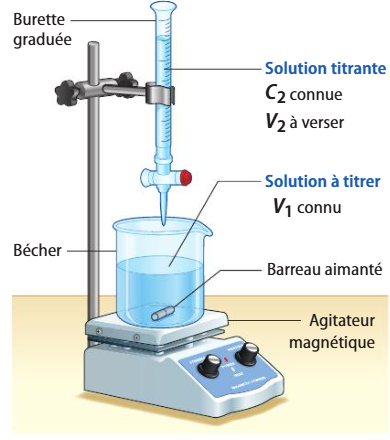
\includegraphics[width=\textwidth]{images/Dosage.png}}
\end{minipage}%



\item \textbf{Titrage colorimétrique}

\begin{minipage}{.96\textwidth}%
\cadreblanc{40}
\end{minipage}% 



\item \textbf{Titrage pH-métrique de l'acide chlorhydrique par la soude}

\begin{minipage}{.96\textwidth}%
\cadreblanc{40}
\end{minipage}% 





\begin{minipage}{.96\textwidth}%
\cadreblanc{40}
\end{minipage}% 

\end{fleche}
\end{document}